\def\year{2018}\relax
%File: formatting-instruction.tex
\documentclass[letterpaper]{article} %DO NOT CHANGE THIS
\usepackage{aaai18}  %Required
\usepackage{times}  %Required
\usepackage{helvet}  %Required
\usepackage{courier}  %Required
\usepackage{url}  %Required
\usepackage{graphicx}  %Required
\usepackage{mwe} %minipage
\usepackage{floatrow}
\frenchspacing  %Required
\usepackage[utf8]{inputenc} % allow utf-8 input
\usepackage[T1]{fontenc}    % use 8-bit T1 fonts
\usepackage{hyperref}       % hyperlinks
\usepackage{url}            % simple URL typesetting
\usepackage{booktabs}       % professional-quality tables
\usepackage{amsfonts}       % blackboard math symbols
\usepackage{nicefrac}       % compact symbols for 1/2, etc.
\usepackage{microtype}      % microtypography

\usepackage{amsmath}
\usepackage{subcaption}
\usepackage{mathrsfs} 
\usepackage{cancel}
\usepackage{amsfonts}
\usepackage[titletoc,title]{appendix}
\usepackage{floatrow}
\usepackage[table]{xcolor}
\usepackage[draft]{todonotes}   % notes showed

% \newcommand{\todo}[2][]{}
% \usepackage{titling}
% \setlength{\droptitle}{-10pt}

\usepackage[]{algorithm2e}
\usepackage{framed}
\newcommand{\papertext}[1]{#1}
\newcommand{\techreport}[1]{}
\newcommand{\agp}[1]{\textcolor{magenta}{Aditya: #1}}
\newcommand{\dor}[1]{\textcolor{blue}{Doris: #1}}
\newcommand{\ads}[1]{\textcolor{green}{Akash: #1}}
% Hide
% \newcommand{\agp}[1]{\textcolor{magenta}{}}
% \newcommand{\dor}[1]{\textcolor{blue}{}}
% \newcommand{\ads}[1]{\textcolor{green}{}}
\setcounter{secnumdepth}{2}

\usepackage{amsopn}
\DeclareMathOperator*{\argmax}{arg\,max}

\newcommand{\sampar}[1]{\vspace{3pt}\noindent{\bf #1}}
\newcommand{\subheading}[1]{\vspace{3pt}\noindent{\bf #1}\\\noindent}

\newcommand{\ta}[1]{\vspace{-3pt}\begin{framed}\vspace{-5pt}\noindent\textit{\underline{Takeaway:} #1}\vspace{-5pt}\end{framed}\vspace{-3pt}}
% usage:   \ta{takeaway text}
\newcommand{\stitle}[1]{\noindent \textbf{#1}}
\newcommand{\takeawaywithqn}[2][]{\vspace{-3pt}\begin{framed}\vspace{-5pt}\noindent\textit{{\bf #1} #2}\vspace{-5pt}\end{framed}\vspace{-3pt}}
% usage:    \ta[question]{takeaway}

\setlength{\pdfpagewidth}{8.5in}  %Required
\setlength{\pdfpageheight}{11in}  %Required
%PDF Info Is Required:
  \pdfinfo{
      /Title (2018 Formatting Instructions for Authors Using LaTeX)
          /Author (AAAI Press Staff)}


\title{Quality Evaluation Methods for Crowdsourced Image Segmentation}
\setlength\titlebox{1.5in}   %squish author title height 
           % The \author macro works with any number of authors. There are two
           % commands used to separate the names and addresses of multiple
           % authors: \And and \AND.
           %
           % Using \And between authors leaves it to LaTeX to determine where to
           % break the lines. Using \AND forces a line break at that point. So,
           % if LaTeX puts 3 of 4 authors names on the first line, and the last
           % on the second line, try using \AND instead of \And before the third
           % author name.
           \begin{document}
           \title{Quality Evaluation Methods for Crowdsourced Image Segmentation}
           \author{Doris Jung-Lin Lee, Akash Das Sarma, Aditya Parameswaran}
           \maketitle
           \begin{abstract}
           Instance-level image segmentation provides rich information crucial for scene understanding in a variety of real-world applications. In this paper we propose and evaluate several crowdsourced algorithms, including novel worker-aggregation based algorithms and retrieval-based methods based on prior work, for the image segmentation problem. We characterize the different types of worker errors observed, and present a clustering algorithm that is able to capture semantic errors and filter workers with different semantic perspectives. We demonstrate that aggregation-based algorithms attain better performance than existing retrieval-based approaches, while scaling better with increasing numbers of collected worker segmentations. 
           % Most large-scale image segmentation efforts such as MSCOCO have relied on computing a Jaccard metric against ground truth and retrieving the segmentation provided by the best worker. 
           \vspace{-10pt}
          \end{abstract}
               
          %!TEX root = main.tex
\vspace{-10pt}
\section{Introduction\label{sec:intro}}
Precise, instance-level object segmentation is crucial for identifying and tracking objects in a variety of real-world emergent applications of autonomy, including robotics~\cite{Natonek1998}, image organization and retrieval~\cite{Yamaguchi2012}, and medicine~\cite{Irshad2014}. To this end, there has been a lot of work on employing crowdsourcing to generate training data for segmentation, including Pascal-VOC~\cite{Everingham15}, LabelMe~\cite{Torralba2010}, OpenSurfaces~\cite{bell15minc}, and MS-COCO~\cite{Lin2012}. Unfortunately, raw data collected from the crowd is known to be noisy due to varying degrees of worker skills, attention, and motivation~\cite{bell14intrinsic,MDWWelinder2010}. 
\par To deal with these challenges, many have employed heuristics indicative of crowdsourced segmentation quality to pick the best worker-provided segmentation~\cite{Sorokin2008,Vittayakorn2011}. Unfortunately, this approach ends up discarding the majority of the worker segmentations and is limited by what the best worker can do. In this paper, we introduce a novel class of aggregation-based methods that incorporates portions of segmentations from multiple workers into a combined one. To our surprise, despite its intuitive simplicity, we have not seen this class of algorithms described or evaluated in prior work. We evaluate this class of algorithms against existing retrieval-based methods described in Section~\ref{sec:related}. \changes{Our analysis of common worker errors in crowdsourced segmentation shows that workers can often annotate around the wrong semantic objects, resulting in large portions the object being erroneously included or excluded from the resulting segmentation. To this end, we propose a clustering-based preprocessing technique that resolves such errors.}%different worker perspectives in multiple segmentations.}
%To resolve semantic ambiguity and mistakes commonly observed in crowdsourced segmentation, we propose a clustering-based preprocessing technique that resolves different worker perspectives in multiple segmentations. 
          %!TEX root = main.tex
\section{Related Work\label{sec:related}}
\begin{figure}[h!]
\centering
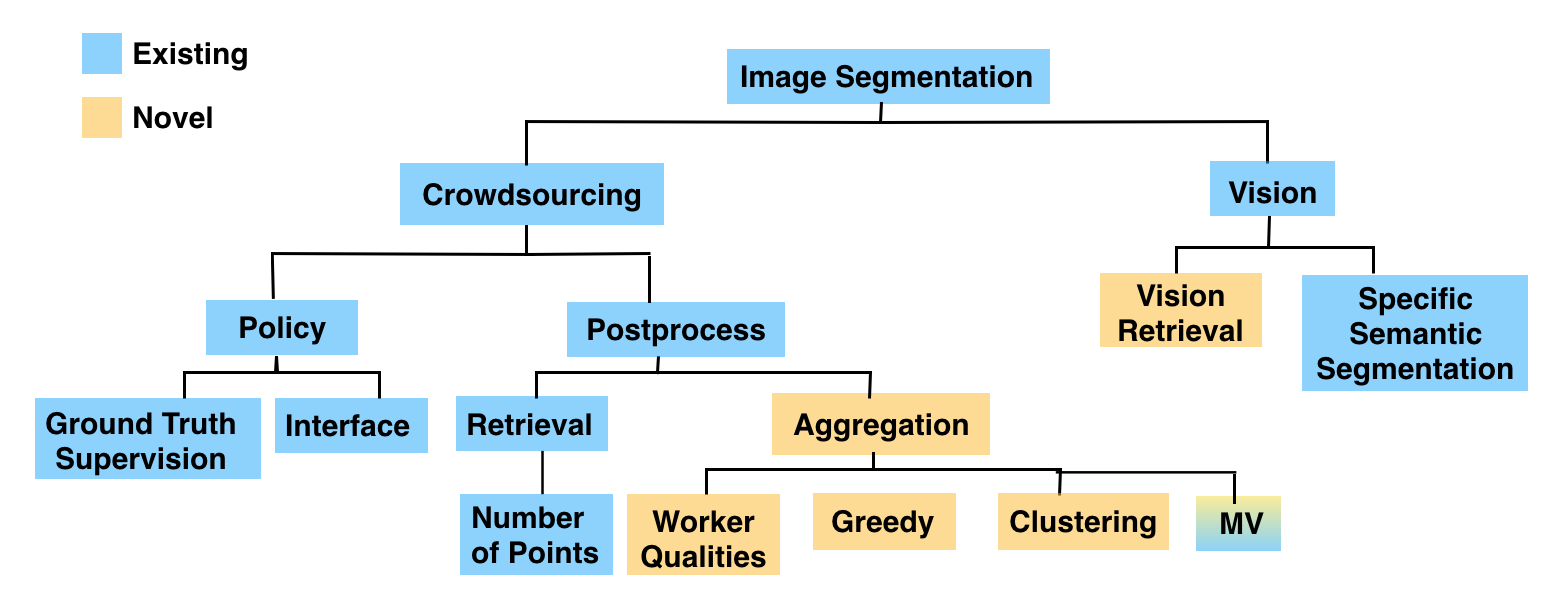
\includegraphics[width=\linewidth]{plots/flowchart.png}
\caption{Flowchart summarizing the classes of existing algorithms for image segmentation (blue) and a novel class of algorithms proposed in this paper (yellow). Majority-vote (MV) is colored both blue and yellow, since a common algorithm in crowdsourcing literature, but have not been extensively applied to crowdsourced image segmentation.}
\vspace{-10pt}
%The crowdsourced approach can be largely classified as retrieval or aggregation-based methods. We further explore hybrid algorithms that makes use of signals that span over multiple categories, described in our technical report.
\label{flowchart}
\end{figure}
%Many large-scale efforts in crowdsourced image segmentation contain little to no information on the quality characterization and evaluation of the collected dataset~\cite{Torralba2010,MartinFTM01,Li2009,Gurari2015}, which indicate the lack of standardized approaches for quality evaluation. 
As shown in Figure \ref{flowchart}, quality evaluation methods for crowdsourced segmentation can be largely classified into two categories:

\stitle{Retrieval-based methods} seek to pick the ``best'' worker segmentation based on some scoring criteria that evaluates the quality of each segmentation, including the use of vision information~\cite{Vittayakorn2011,Russakovsky2015}, expectation-maximization (EM) approaches for bounding box quality estimation~\cite{MDWWelinder2010}, and click-stream behavior \cite{Cabezas2015,Sameki2015,Sorokin2008}.

\stitle{Aggregation-based methods} use multiple worker segmentations to produce a single combined segmentation. %Our paper formulate a novel ``tiles'' approach for aggregation methods that operates on discrete non-overlapping units composed of all worker segmentations overlaid on top of each other. 
\ads{reword a bit to emphasize difference from retrieval; Aggregation-based methods combine multiple worker segmentations to produce a final segmentation, and are not restricted by any single worker segmentation.}
Aggregation-based majority vote have been introduced in Sameki et al. (\citeyear{Sameki2015}) as a way for aggregating expert segmentations to obtain a ground truth segmentation for evaluation purposes. \ads{Not clear how what they did is different from us---important to reword so that novelty of our aggregation methodology (and MV algo in particular) is not questioned.}

%specialized segmentation interfaces or workflows that ensures that the annotations collected are of high quality, including 
Orthogonal methods to improve segmentation quality include periodic verification workflows~\cite{Lin2014,Everingham15}, specialized segmentation interfaces~\cite{Song2018}, and vision-based supervision of crowdsourced segmentation\cite{Russakovsky2015,Gurari2016}. Our paper do not compare against these methods since they are not easily reproducible and could be used for quality improvement on top of any of the algorithms described in this paper.  %Since these policy-based methods are interface-dependent, require expensive expert-drawn ground-truth annotations or vision information, the results are not easily reproducible. In addition, the segmentations collected by the simple click-and-draw interface in many of the large scale segmentation efforts can not be improved with this technique as a post-processing method. Due to the lack of reproducibility, our paper do not compare against these policy-based methods in extensive details.


          \section{Preliminaries}
\subsection{Data \& Goals}
We collected crowdsourced segmentation data from Amazon Mechanical Turk where each HIT consisted of one segmentation task for a specific pre-labeled object in the image. There were a total of 46 objects in 9 images from the MSCOCO dataset~\cite{Lin2014}. For each object, we collected segmentation masks from a total of 40 workers. As shown in Figure \ref{interface}, each task contains a semantic keyword and a pointer indicating the object to be segmented. These tasks represent a diverse set of task difficulty (different levels of clutteredness, occlusion, lighting) and levels of task ambiguity. %Given a raw 
\subsection{Evaluation Metrics}
\par Evaluation metrics used in our experiment measures how well the final segmentation (S) produced by these algorithms compare against ground truth (GT). The most common evaluation metric used in literature are area-based methods which take into account the intersection, $IA=area(S\cup GT)$, or union, $UA=area(S\cap GT)$, between the user and the ground truth segmentations. Specifically, we use
    $\text{Precision (P)} = \frac{IA(S)}{area(S)}$, 
    $\text{Recall (R)} = \frac{IA(S)}{area(GT)}$, and 
    $\text{Jaccard (J)} = \frac{UA(S)}{IA(S)}$
    metrics to evaluate our algorithms.
 \techreport{\par A sub-sampled dataset was created from the full dataset to determine the efficacy of these algorithms on varying number of worker responses. Every object was randomly sampled worker with replacement. For small worker samples, we average our results over larger number of batches than for large worker samples (which have lower variance, since the sample size is close to the original data size).}
          \section{Precision-focused algorithms}%: Aggregation v.s. Retrieval Comparison}
% \subsection{Retrieval-based methods}
% This class of algorithms tries to identify good and bad workers, and then chooses the best worker segmentation as the output segmentation. In this paper, we look at two different ways of ranking workers and choosing the best worker. First, we use the {\em number of control points}, i.e. number of vertices in a worker's segmentation polygon to rank workers. This is a ranking scheme that~\cite{Vittayakorn2011} showed performs well in practice. Intuitively, workers that have used a larger number of points are likely to have been more precise, and provided a more complex and accurate segmentation. Other heuristic ranking scheme is described in more detail in our technical report~\cite{segmentation-tr}.
\begin{figure}[h!]
\vspace{-10pt}
\centering
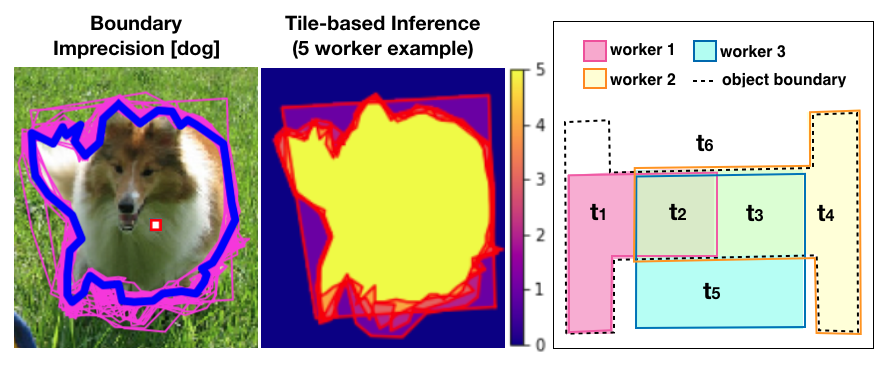
\includegraphics[width=0.8\textwidth]{plots/precision_issue_tile_example.png}
\caption{Left: Pink boundaries shows worker segmentations and blue delineates the ground truth. Right: Segmentation boundaries drawn by five workers shown in red. Overlaid segmentation creates a masks where the color indicates the number of workers who voted for the tile region.}
\label{tile_demo}
\end{figure}
\vspace{-10pt}
At the heart of our aggregation techniques is the ``tile'' data representation, where we logically overlay all workers' segmentations on top of each other, as illustrated in Figure \ref{tile_demo} right, to create non-overlapping discrete tile units. The intuition here is that by splitting the image into tiles, we get finer granularity information than by looking at complete segmentations. This also allows us to aggregate data from multiple workers rather than having to choose a single worker bounding box---enabling the opportunity to choose partial segmentations by fixing one worker's errors via the help from another worker's segmentation. Now, we will describe several algorithms for picking a good set of tiles.

\stitle{Aggregation: Majority Vote Aggregation (MV)} 
\par \noindent Include tiles in the output segmentation if and only if the tile is covered by at least 50\% of all worker segmentations.

\stitle{Aggregation: Expectation-Maximization (EM)}
\par \noindent Unlike MV, which assumes that all workers performs uniformly, EM approaches use worker quality models to infer the likelihood that a tile is part of the ground truth segmentation. The EM algorithm simultaneously estimate both worker qualities and tile likelihoods as hidden variables. Details of the formal derivation and three worker quality models that we have developed can be found in our technical report.

\stitle{Aggregation: Greedy Tile Picking (greedy)} 
\par \noindent Using tile probabilities from EM to estimate intersection area between ground truth and tile, then greedily pick tiles with the largest intersection area ratio until Jaccard score begins to decrease (effectively picking the largest and most probable tiles that should be included first). The Jaccard score is computed between the merged output from the selected set of tiles and MV segmentation.

\stitle{Retrieval: Number of Control Points (num pts)}
\par \noindent Pick the worker segmentation with the largest number of control points around the segmentation boundary (i.e. most precise drawing) as the output segmentation.
          %!TEX root = main.tex
\section{Perspective Resolution in Crowdsourced Image Segmentation}
\subsection{Worker Clustering}
Our clustering-based approach is based on the intuition that workers with similar perspectives  will have segmentations that are closer to each other, while workers with different perspectives from each other will have segmentations that differ from each other. We capture the similarity between a pair of workers by computing the Jaccard score between their segmentations and perform {\em spectral clustering} to separate workers into clusters. Figure \ref{cluster_example} illustrates how spectral clustering is capable of dividing the worker responses into clusters with meaningful semantic associations, reflecting the crowd's diversity of perspectives in completing same task.
    \begin{figure}[ht!]
      \centering
      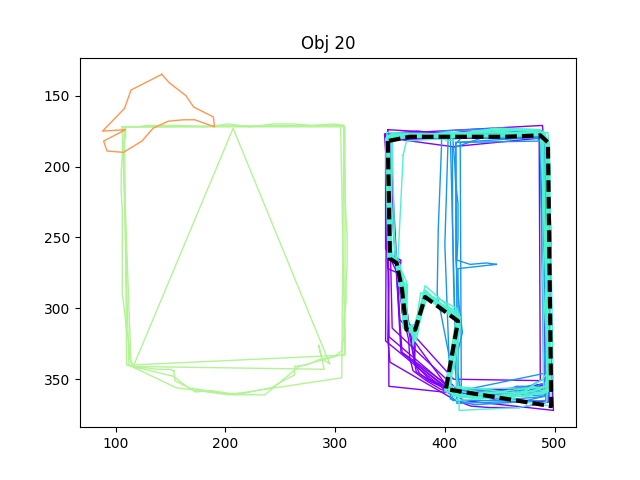
\includegraphics[width=\textwidth]{plots/20.png}
      \caption{Example image showing clustering performed on the same object from Figure \ref{error_examples}.}
      \label{cluster_example}
    \end{figure}
\par Clustering results can also be used as a preprocessing step to any of the quality evaluation algorithms by keeping only the segmentations that belong to the largest cluster, which is typically free of any semantic errors. As shown in Table~\ref{statsTable}, on average, clustering generally results in an increase the resulting algorithmic performance. Since the ground-truth supervised variants are already free of semantic ambiguity and errors, there is minimal improvement resulting from clustering. %In particular, we see a greater improvement with clustering preprocessing for algorithms that are not very robust in resolving semantic errors or ambiguity, such as for the \texttt{num pts} retrieval algorithm, than compared to the aggregation-based methods. 
\par Clustering offers an additional benefit of preserving worker's semantic intentions in the case where there are multiple instances of different errors. For example, in Figure \ref{cluster_example}, the mistakened clusters included semantic concepts ``monitor'' and ``turtle''. While these are considered \textit{bad} annotations for this particular task, this cluster of annotation can provide more data for another semantic segmentation task ``monitor''. A potential direction of future work includes adding an additional crowdsourcing task for semantic labelling of clusters (which is cheaper and more accurate than segmentation) to enable reuse of annotations across objects and lower the cost of data collection. 
          \section{Conclusion \& Future Work}
In this paper, we identified three different types of errors for crowdsourced image segmentation, and developed a clustering-based method capture the semantic diversity caused by differing worker perspectives. Moreover, we introduced novel aggregation-based methods that performed better when compared to existing retrieval-based methods.
\par Given the success of aggregation-based methods, our future work investigates why and how our EM and greedy approaches differ from majority vote. Our preliminary studies show that worker qualities are good indicators of actual Jaccard of worker segmentations with ground truth and that the greedy algorithm is capable of achieving close-to-perfect segmentation accuracy with ground truth information. We have also explored using vision information to improve these algorithms. Bridging the gap between our current approach to the maximum potential of aggregation-based methods can result in more accurate and perspective-aware crowdsourced segmentation outputs in the future.
\bibliographystyle{named}
\bibliography{reference}
\end{document}
